%! Author = spruhs
%! Date = 25.02.25

% Preamble
\documentclass[11pt]{article}

% Packages
\usepackage[utf8]{inputenc}
\usepackage[T1]{fontenc}
\usepackage[ngerman]{babel}
\usepackage{graphicx}
\usepackage{tocloft}
\usepackage{appendix}
\usepackage{csquotes}
\usepackage[
    backend=biber,
    style=alphabetic,
]{biblatex}
\usepackage{color}
\addbibresource{literaturverzeichnis.bib}

% Document
\begin{document}

    \begin{titlepage}
        \centering
        {\scshape\LARGE Seminar 1908 Moderne Programmiertechniken und -Methoden -Sommer 2025 \par}
        \vspace{1cm}
        {\huge\bfseries Kotlin statt Java\par}
        \vspace{1.5cm}
        {\scshape\Large Fabian Spruhs\par}
        {\scshape fabian@spruhs.com\par}
        \vspace{2cm}
        {\Large\itshape Studiengang Bachelor Informatik\par}
        \vspace{2cm}


        {\large \today\par}
    \end{titlepage}

    \tableofcontents
    \newpage

    \section{Einleitung}
    \section{Kurzvorstellung Java}
    \subsection{Übersicht}
    \begin{itemize}
        \item \textbf{Erscheinungsjahr:} 1995
        \item \textbf{Entwickler:} Sun Microsystems
        \item \textbf{Entwickler ab 2009:} Oracle Corporation
        \item \textbf{Programier paradigmen:} objektorientiert
        \item \textbf{Aktuelle LTS version:} 21
    \end{itemize}


    \subsection{Technischer Hintergrund}
    Java ist eine Programiersprache die im von Sun Microsystem entwickelt wurde un im Jahre 1995
    veröffentlicht wurde. Sie unterstütztdie objektorientierte programier Paradigma. Ihre Robustheit
    und die individuellen Einsatzmöglichkeiten macht Java für die Industrie interessant.\\
    Eine zentrale eigenschaft von Java ist es, dass der Code zunächst einmal in Bytecode kompiliert wird.
    Der Bytecode kann dann auf einer viertuellen Laufzeitumgebung, der Java viertuel Machiene (JVM) ausgeführt werden.
    Dadurch ist der Javacode nicht an eine bestimmte Prozessorarchitektur oder an ein bestimmtes Betriebssystem gebunden.
    Diese Platformunabhängigkeit ist grosser Vorteil von Java den viele andere Sprachen über die Zeit übernommen haben.
    Die JVM bietet dabei automatische dienste wie starke typisierung, einen Garbag-collect oder das verwalten
    von Threads an.\cite[51 - 54]{insel}
    Grundsätzlich ist die Ausführung von Java code auch ohne die JVM möglich. Dazu kann Java Code in Java Nativs kompiliert werden.
    Diese können dann nur auf bestimmten System ausgeführt werden.


    \subsection{Verbreitung}
    Der TIOBE Index ist ein Index der die Popularität und die Verbreitung von Programiersprachen monatlich misst\cite{tiobe}.
    Nach diesem Index gehört Java zu einem der meist verbreitesten Sprachen überhaupt. Wie man der Entwicklung in Abbildung \ref{fig:entwicklung-tiobe}
    entnehmen kann, war fast 2 Jahrzehnte unter den Top 3 der relevantesten Prgramiersprachen weltweit. In den letzten Jahren hat die
    popuarität von Java zwar etwas abgenommen, gehört aber weiterhin zu einem der Relevantesten Sprachen. Im Februar 2025 war Java auf
    Platz 3 des TIOBE Index, siehe Abbildung \ref{fig:tiobe-2025}.\\
    Weltweit sind sehr viele Anwendungen in Java geschrieben. Weiterhin existieren für Java unzählige von Bibliotheken, Packeten, Frameworks und Fachliteratur.
    Weiterhin gibt es unzählige Java Entwickler und Communitys mit einem reichhaltigen Wissenschatz im Bereich Java.
    Alleine bei Maven existieren über 2.800 repositories mit über 52 million Paketen für Java \cite{maven}.
    Dieser Grosse Infrastruktur ist ein weiterer Vorteil von Java.

    \subsection{bla bla 2}
        more content

    \printbibliography[
        heading=bibintoc,
        title={Literaturverzeichnis}
    ]

    \appendix
    \section{Anhang}

    \begin{figure}[h]
        \centering
        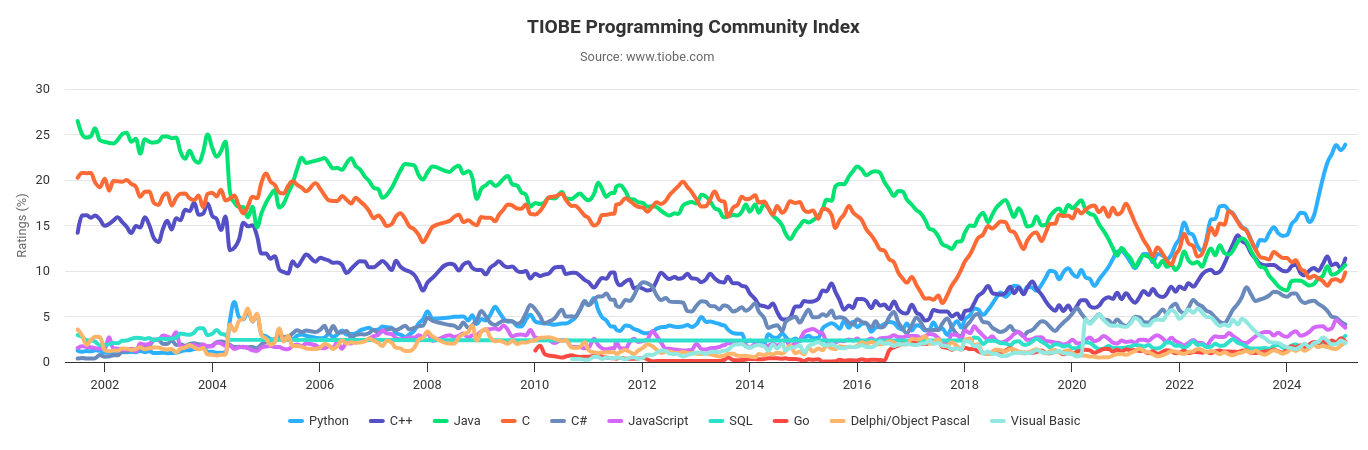
\includegraphics[width=0.8\textwidth]{pictures/Screenshot 2025-02-26 at 19-53-49 TIOBE Index - TIOBE}
        \caption{Entwicklung Tiobe Index 2002 - 2024 vom 26.02.2025 }
        \label{fig:entwicklung-tiobe}
    \end{figure}

    \begin{figure}[h]
        \centering
        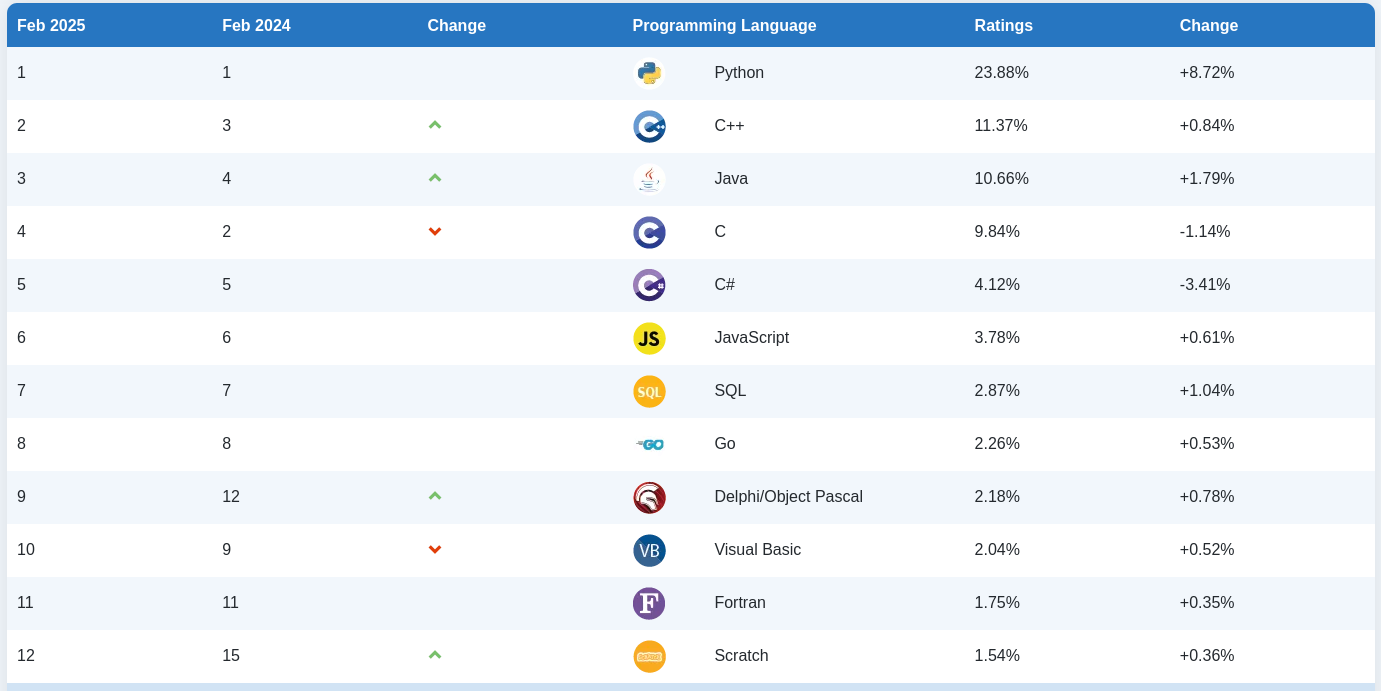
\includegraphics[width=0.8\textwidth]{pictures/Screenshot 2025-02-26 at 19-54-42 TIOBE Index - TIOBE}
        \caption{Tiobe Index Februar 2025 vom 26.02.2025}
        \label{fig:tiobe-2025}
    \end{figure}

    \cite{insel}
    \cite{kotlin-handbuch}



\end{document}